\section{Zielsetzung}
\label{sec:Zielsetzung}
Ziel dieses Versuches ist es, die Funktionsweise eines Lock-In-Verstärkers anhand verschiedener Probeschaltungen 
kennenzulernen. Dafür werden sowohl verrauschte, als auch unverrauschte Eingangssignale verwendet und ausgewertet.

\section{Theorie}
\label{sec:Theorie}
Ein Lock-In-Verstärker ermöglicht es stark verrauschte Signale bis zu einem Gewissen Grad zu entrauschen. Dazu wird
das verrauschte Eingangssignal $U_{\symup{sig}}$ zunächst durch einen Bandpassfilter von Frequenzen $\omega$, die höher 
oder tiefer als die Zielfrequenz $\omega_{0}$ sind, bereinigt. Anschließend wird das Eingangssignal $U_{\symup{sig}}$ mit 
einem Referenzsignal $U_{\symup{ref}}$ selber Frequenz $\omega_{0}$ und Phase $\varphi$ multipliziert, um weiteres Rauschen 
zu unterdrücken. Dies bewirkt auch eine Gleichrichtung des Eingangssignals. Mithilfe eines Tiefpassfilters mit 
Zeitkonstante~$RC >> \frac{1}{\omega_{0}}$ werden Frequenzen $\omega$, die nicht der Zielfrequenz $\omega_{0}$ entsprechen,
nahezu vollständig herausgefiltert. Darüber hinaus integriert der Tiefpassfilter das Eingangssignal $U_{\symup{sig}}$.

\begin{figure} [H]
    \centering
    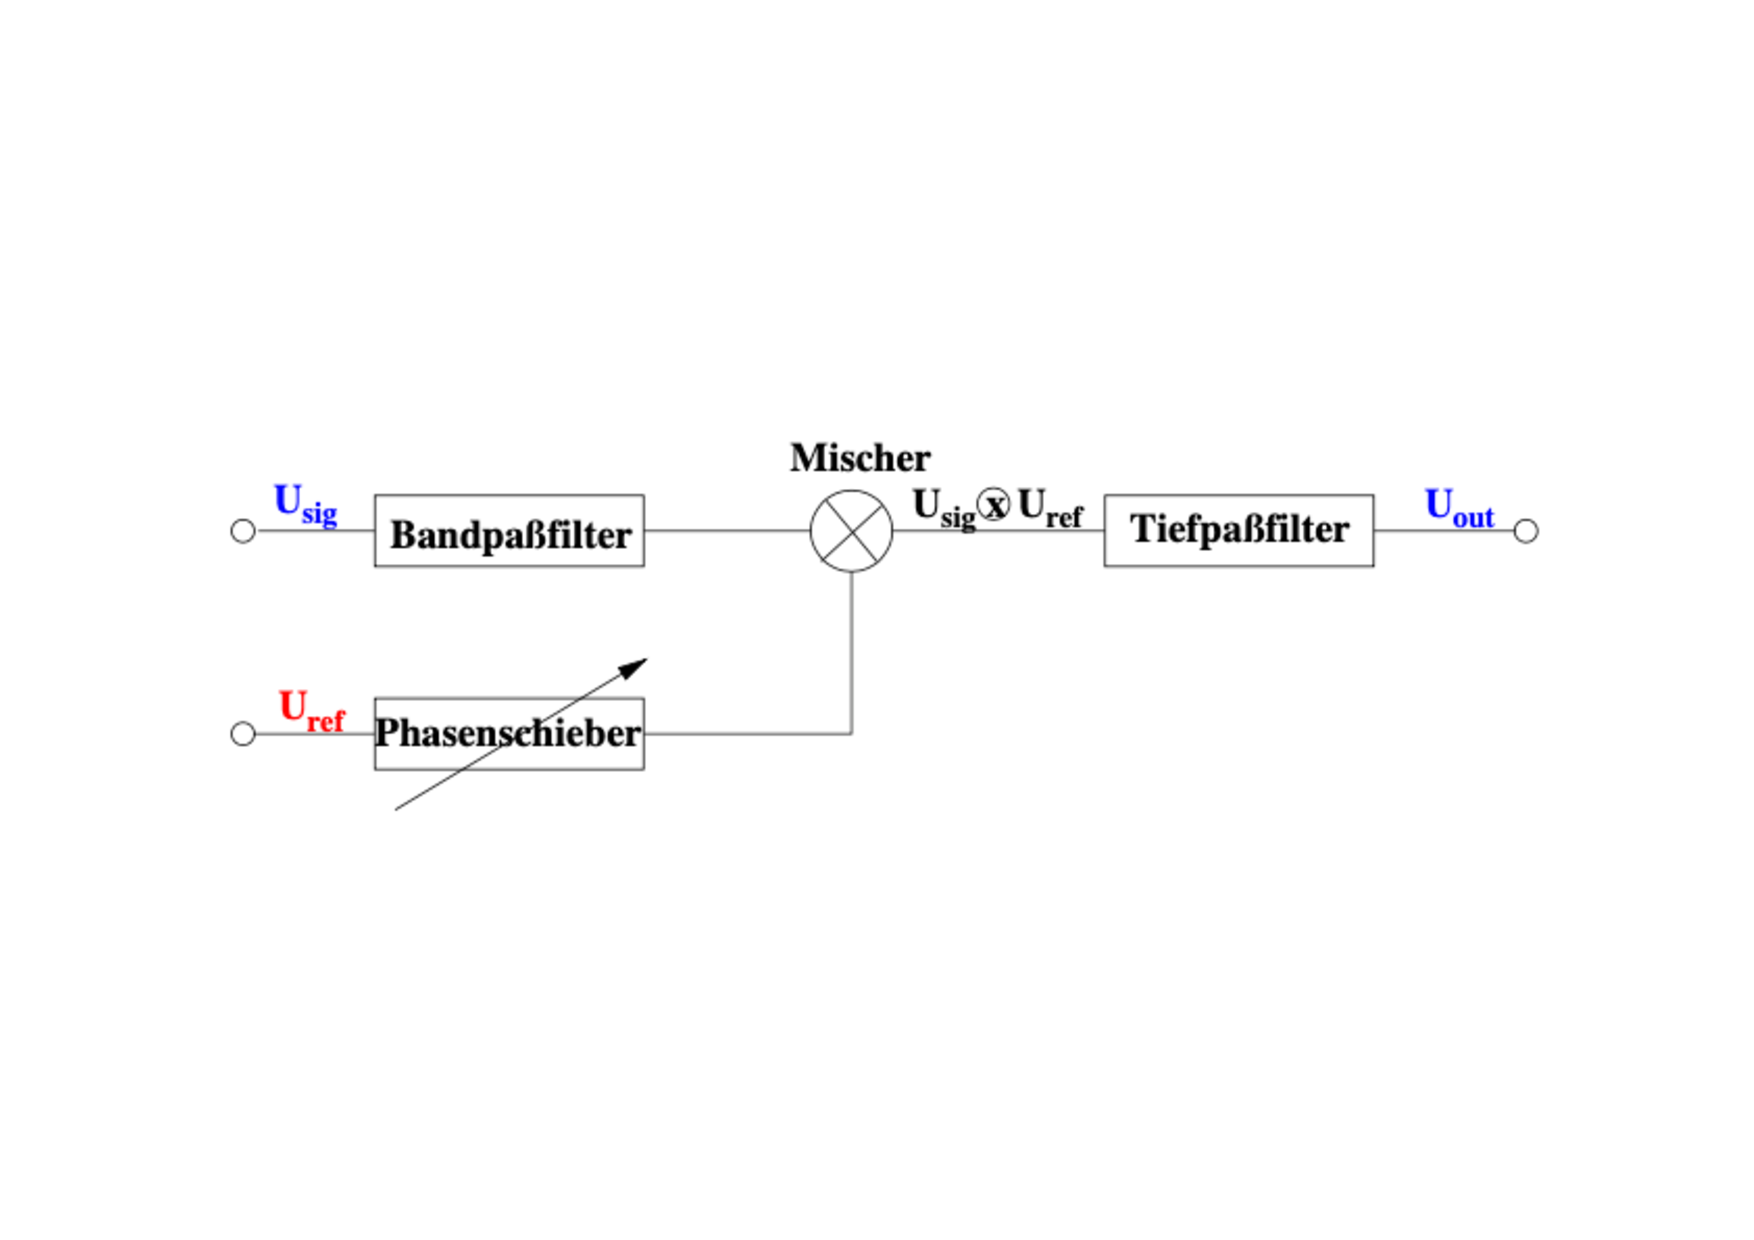
\includegraphics[height=5cm]{content/Bilder/Aufbau_LockInVerstaerker.pdf}
    \caption{Schematischer Aufbau eines Lock-In-Verstärkers.\cite{v303}}
    \label{fig:Aufbau}
\end{figure}

\begin{figure} [H]
    \centering
    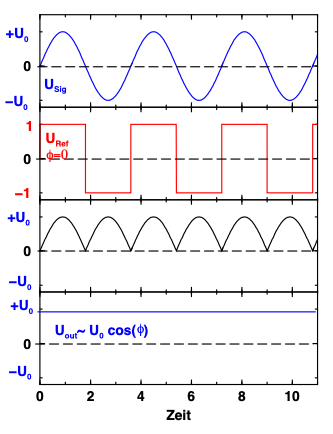
\includegraphics[height=10cm]{content/Bilder/Signalverlaeufe.png}
    \caption{Sinusförmiges Eingangssignal mit rechteckigem Referenzsignal und resultierendem %
    Ausgangssignal.\cite{v303}}
    \label{fig:Signalverlaeufe}
\end{figure}

Es ergibt sich, folgender Zusammenhang
\begin{equation}
    U_{\symup{out}} = \frac{2}{\symup{\pi}}U_{\symup{0}}\symup{cos}(\symup{\Delta}\varphi).
    \label{eq:Ausgangssignal Proportionalitaet}
\end{equation}
Folglich wird das Ausgangssignal maximal bei einer Phasenverschiebung $\symup{\Delta}\varphi = k\pi$ mit einem $k$ aus den ganzen
Zahlen $\mathbb{Z}$.
